\documentclass[conference]{IEEEtran}
\IEEEoverridecommandlockouts
% The preceding line is only needed to identify funding in the first footnote. If that is unneeded, please comment it out.
\usepackage{cite}
\usepackage{amsmath,amssymb,amsfonts}
\usepackage{algorithmic}
\usepackage{graphicx}
\usepackage{textcomp}
\usepackage{xcolor}
\def\BibTeX{{\rm B\kern-.05em{\sc i\kern-.025em b}\kern-.08em
		T\kern-.1667em\lower.7ex\hbox{E}\kern-.125emX}}
\begin{document}
	
	\title{Report 1}
	
	\author{\IEEEauthorblockN{1\textsuperscript{st} Ali Ramezanzadeh}
		\IEEEauthorblockA{\textit{dept. of Electrical Engineering} \\
			\textit{Amirkabir University of Technology}\\
			Tehran, Iran\\
			ali.ramezan@aut.ac.ir}
		\and
		\IEEEauthorblockN{2\textsuperscript{nd} Arian Abdollahi}
		\IEEEauthorblockA{\textit{dept. of Electrical Engineering} \\
			\textit{Amirkabir University of Technology}\\
			Tehran, Iran\\
			arian.abdollahi@aut.ac.ir}
		\and
		\IEEEauthorblockN{3\textsuperscript{rd} Sina Shah Mohammadi}
		\IEEEauthorblockA{\textit{dept. of Electrical Engineering} \\
			\textit{Amirkabir University of Technology}\\
			Tehran, Iran\\
			alisinashahmohammadi@aut.ac.ir}}
	
	\maketitle

	
	\section{Introduction}
In this experiment, we want to design a lead and lag controller for an flexible joint robot.\newline
A flexible joint robot is a type of robot designed with joints that offer some degree of flexibility, compliance, or elasticity, distinguishing them from rigid robots. These robots incorporate elements like springs, elastic actuators, or specially designed mechanisms to allow controlled movement with some give or deformation at the joints. 

	\begin{figure}[htbp]
	\centerline{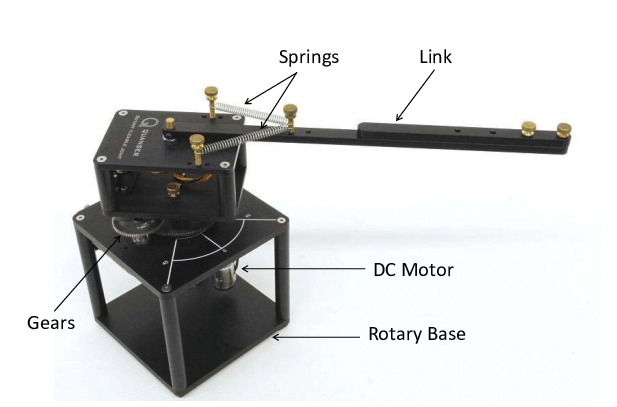
\includegraphics[width=0.7\linewidth]{1.jpg}}
	\caption{Flexible Joint Robot}
	\label{fig1}
\end{figure}

	\section{Mathematical Modeling}
We use the following diagram to derive the mathematical model of the system:

\begin{figure}[htbp]
	\centerline{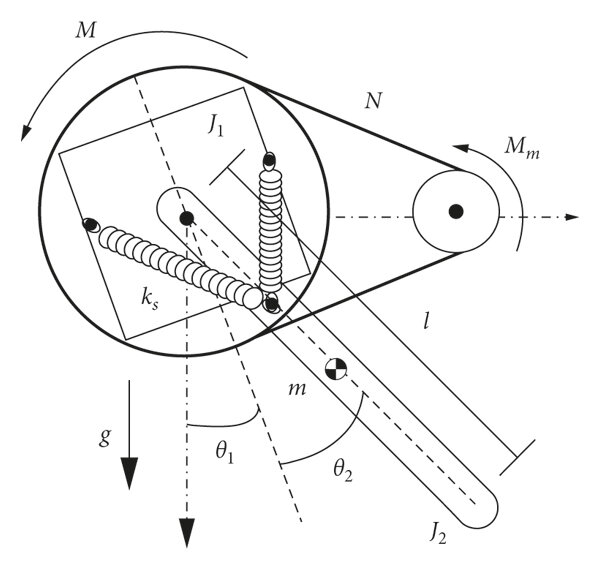
\includegraphics[width=0.7\linewidth]{2.jpg}}
	\caption{Flexible Joint Robot Model}
	\label{fig1}
\end{figure}

Using Lagrange-Hamilton, we arrive at the following equations.


\begin{equation}
	J_{eq} \ddot{\theta}+ J_{Arm}( \ddot{\theta}+\ddot{\alpha})=T_{output}-B_{eq}\dot{\theta}
\end{equation}


\begin{equation}
J_{Arm}( \ddot{\theta}+\ddot{\alpha})+K_{stiff}\alpha=0
\end{equation}

And we have the torque of a DC motor:

\begin{equation}
	T_{output}=\dfrac{\eta_{m}\eta_{g}K_{g}K_{m}(V_{m}-K_{g}K_{m}\dot{\theta})}{R_{m}}
\end{equation}
The selected state variables are:

\[
X=
\begin{pmatrix}
	\theta \\
	\dot{\theta}\\
	\alpha \\
	\dot{\alpha}\\
\end{pmatrix}
\]


Then, using the solve command in MATLAB, we solve the above equations and obtain the state-space matrices:

\[
A=
\begin{pmatrix}
	0 & 1 & 0 & 0 \\
	0 & {\frac{- (K_m  K_t  n_g  n_m   K_g^2 + B_{eq}  R_m)}{a}} & {\frac{K_{stiff}}{J_{eq}}} & 0 \\
	0 & 0 & 0 & 1 \\
	g &  {\frac{ (K_m  K_t  n_g  n_m   K_g^2 + B_{eq}  R_m)}{a}} & {\frac{-K_{stiff}(J_{arm}+J_{eq})}{J_{eq}J_{arm}}} & 0 \\
\end{pmatrix}
\]

\[
B=
\begin{pmatrix}
	0 \\
	\dfrac{K_{t}K_{g}\eta_{g}\eta_{m}}{J_{eq}R_{m}} \\
	0 \\
	-\dfrac{K_{t}K_{g}\eta_{g}\eta_{m}}{J_{eq}R_{m}} \\
\end{pmatrix}
\]

\[
C=
\begin{pmatrix}
	1 & 0&0 &0  \\
\end{pmatrix}
\qquad D=0
\]


A lag controller is a type of feedback controller used in control systems to improve certain characteristics, primarily focusing on steady-state error and system stability. The term "lag" indicates that the controller introduces a delay or slower response to the system, often through an additional pole in the transfer function:

\begin{equation}
	G_{\text{Lag}} = K_c \left( \frac{s + z_c}{\alpha s + p_c} \right) = K_c \left( \frac{\tau s + 1}{\alpha \tau s + 1} \right)
\end{equation}


Thus:
\[
 \alpha \triangleq \frac{z_c}{p_c} > 1, \quad \tau = \frac{1}{z_c} = \frac{1}{\alpha p_c}
\]


The first step in designing such compensation is to calculate its gain in a way that satisfies the desired steady-state error


\begin{equation}
	K_c = \frac{e_{ss} - e_{\text{plant}}}{e_{ss} - e_{\text{specified}}} = \frac{K_{x-requierd}}{K_{x-plant}}
	\end{equation}

\begin{equation}
	K_x = \lim_{s \to 0} s^N \cdot G(s)
\end{equation}


\begin{equation}
	\phi_m = PM_{desired}-PM+5
\end{equation}


Thus:
\[ K_c = 2.841 \]

\[ Z = 0.483 \quad P = 0.0483\]

this is the bode diagram of the system before applying the lag controller:

\begin{figure}[htbp]
	\centerline{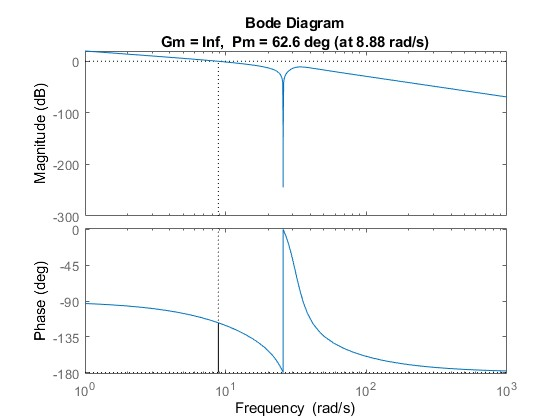
\includegraphics[width=0.9\linewidth]{3.jpg}}
	\caption{System Bode Diagram}
	\label{fig3}
\end{figure}
\newpage
And this is the bode diagram of the system after applying the lag controller:

\begin{figure}[htbp]
	\centerline{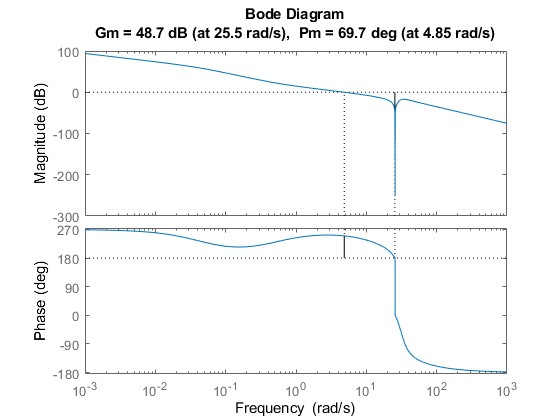
\includegraphics[width=0.9\linewidth]{4.jpg}}
	\caption{System Bode Diagram With Lag Controller}
	\label{fig4}
\end{figure}

	\section{Simulink}
	
	After all we plant the system on simulink. Here is the result:

\begin{figure}[htbp]
	\centerline{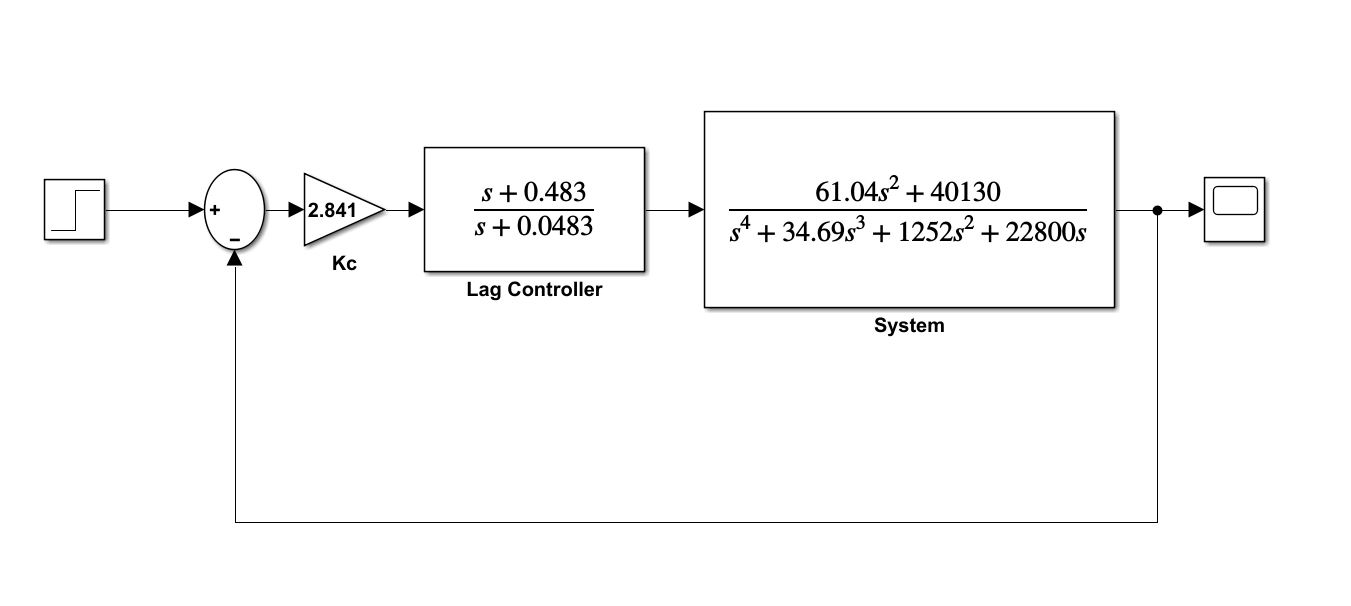
\includegraphics[width=0.9\linewidth]{5.jpg}}
	\caption{System With Lag Controller Simulink}
	\label{fig5}
\end{figure}
And now test our system with lag controller on flexible joint Robot :
\begin{figure}[htbp]
	\centerline{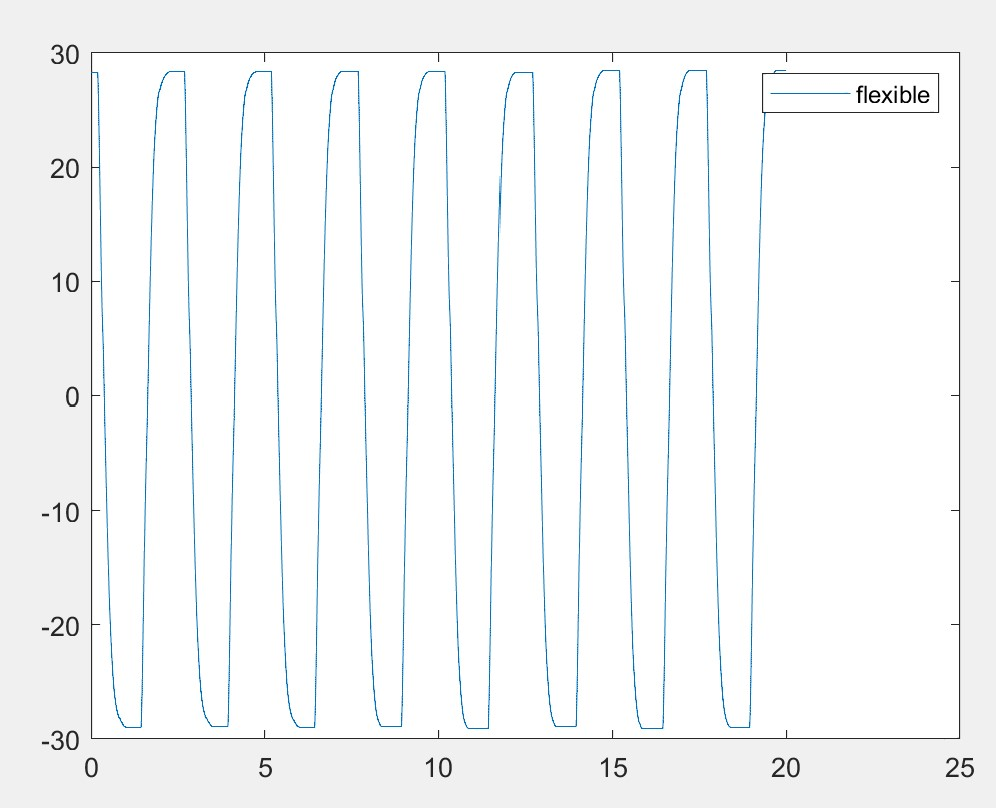
\includegraphics[width=0.7\linewidth]{6.jpg}}
	\caption{Flexible joint robot response }
	\label{fig6}
\end{figure} 

This figure shows that by adding lag to our system,we slow down the system and reduce overshoot,which can be justified considering the features of the lag controller.
\end{document}

